% Method section

% We present our framework for multi-turn model routing. We first formalize the problem (\S\ref{sec:formalization}), then describe our history and model representations (\S\ref{sec:representations}), and finally detail the learning approach (\S\ref{sec:learning}).

\subsection{Problem Formalization}
\label{sec:formalization}

\begin{figure*}[!t]
\centering
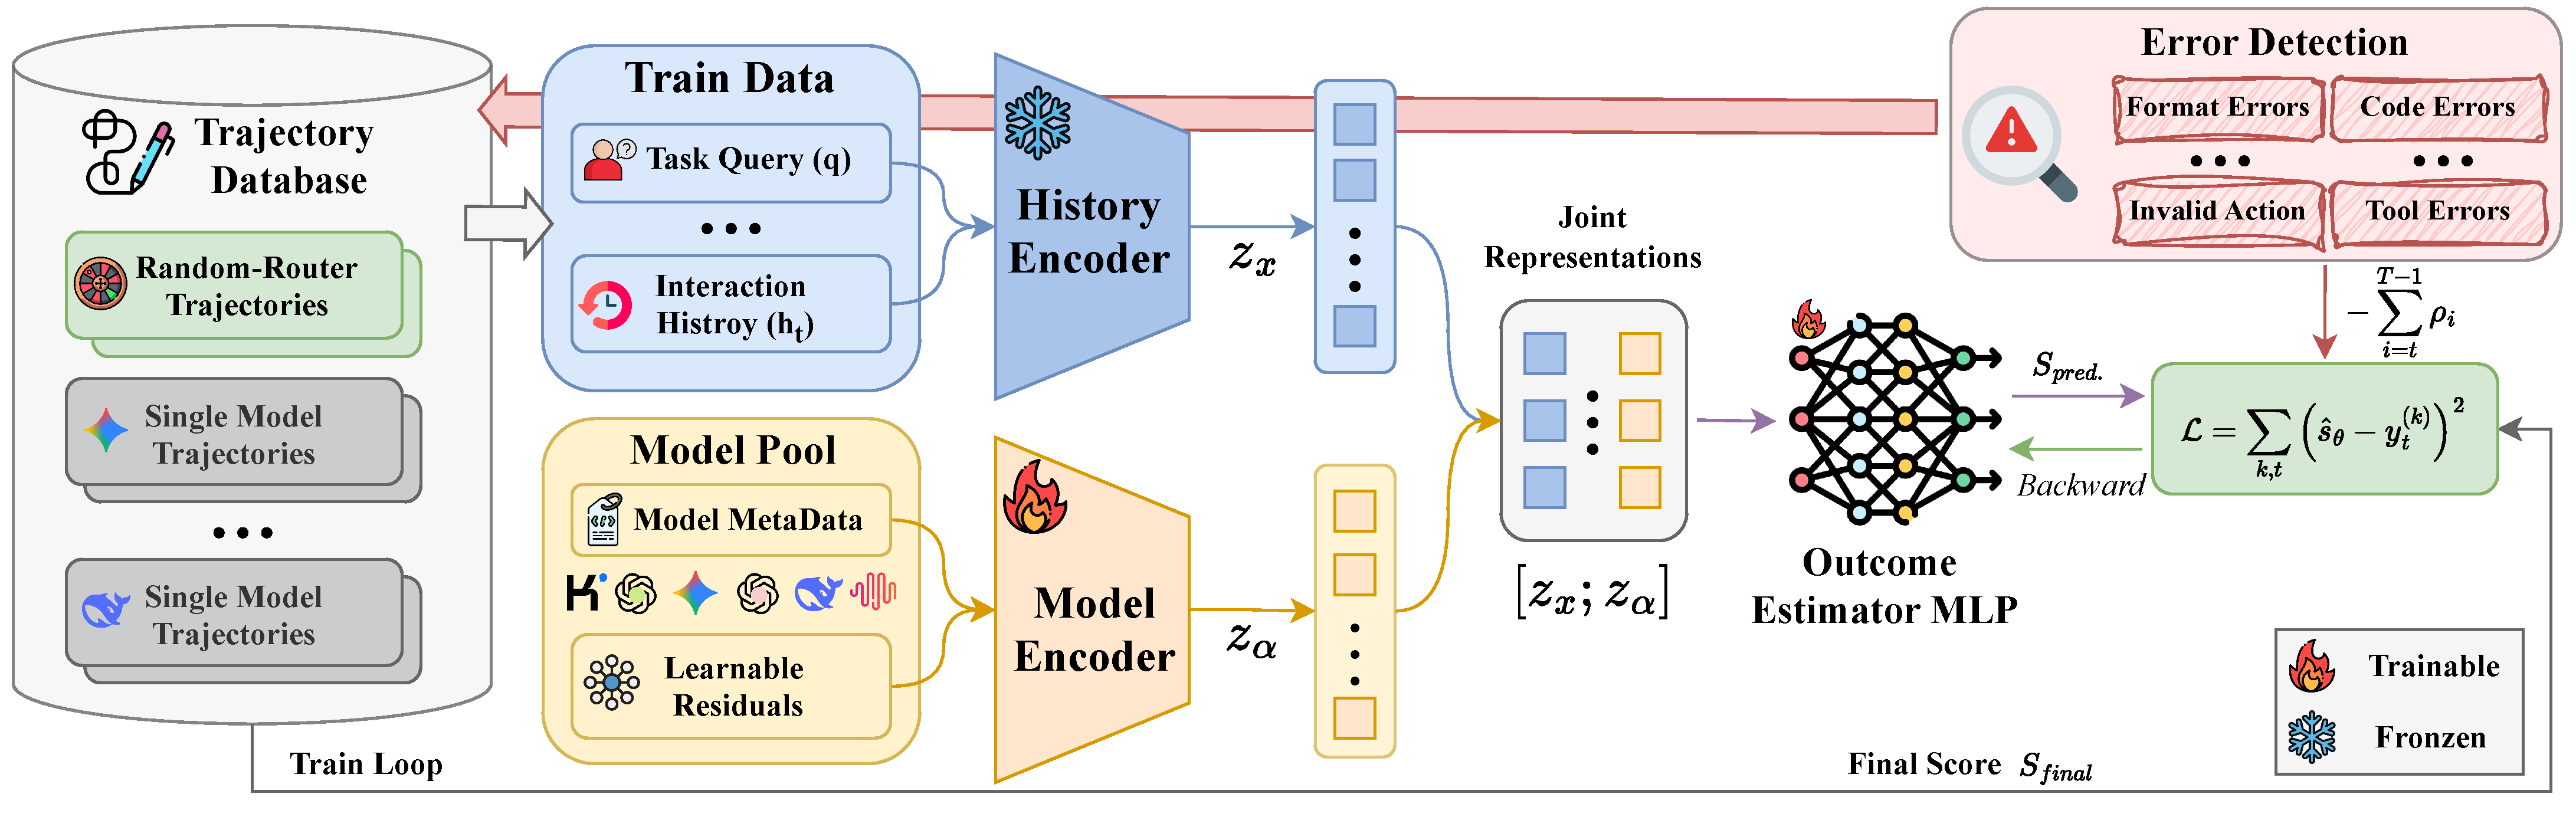
\includegraphics[width=\linewidth]{figures/main-figure.pdf}
\caption{\textbf{Overview of \method.}}
\label{fig:method_overview}
\vspace{-1.0em}
\end{figure*}

Single-turn (episode-level) routing makes one model choice at the start of an episode and keeps it fixed. We study \emph{multi-turn} model routing, where the model choice can change over time.
An episode consists of turns indexed by $t$.
At each turn, a router selects a model $a_t \in \mathcal{A}$ to generate the agent's next output (the router itself may be implemented by an LLM).
A \textbf{turn} is one round of interaction that includes exactly one invocation of the selected model: given the \textbf{history} $h_t$ (task description, dialogue context, and the most recent observation), the selected model produces $y_t \sim p_{a_t}(\cdot \mid h_t)$, and a \textbf{parser} maps $y_t$ to an executable action $u_t=\text{parse}(y_t)$; executing $u_t$ yields the next observation $o_{t+1}$.

The episode ends when the task is completed (as indicated by the environment or by an agent submission), a turn limit is reached, or a cost budget is exhausted. The environment provides a terminal score $S_{\text{final}}$.

\paragraph{Objective.}
We optimize task performance under a per-episode cost budget:
\begin{equation}
\max \; \mathbb{E}\left[S_{\text{final}}\right] \quad \text{s.t.} \quad \sum_{t=0}^{T-1} c_t \le B
\label{eq:objective}
\end{equation}
where $c_t$ is the cost at turn $t$ (computed from token usage and model pricing), $B$ is a per-episode cost budget, and $T\le T_{\max}$ is the episode length (capped by a maximum turn limit). Episodes terminate when the budget is exhausted or the turn limit is reached.

\subsection{Joint History--Model Representations}
\label{sec:representations}

Routing decisions depend on both the interaction history and the chosen model (i.e., the pair $(h_t,a_t)$). We therefore embed history and candidate models separately and then combine them into a joint representation used by the router.

\paragraph{History Encoding.}
We represent the routing history as the task block plus the accumulated interaction context. Concretely, we serialize each example with a fixed template:

\begin{equation}
{\textstyle h_t = [q,\langle u_0,o_1\rangle,\ldots,\langle u_{t-1},o_t\rangle]}
\end{equation}
At implementation time, we do not use a fixed number of retained turns K. Instead, we apply token-budget truncation with a maximum length of 8192 tokens: we always keep the task block and retain the most recent interaction context within the remaining budget, truncating the oldest context first. The serialized history is then encoded by a frozen text encoder $\phi$ to obtain $z_x=\phi(h_t)\in\mathbb{R}^d$. 
% The router input consists only of the current history representation and the candidate-model representation; we do not feed explicit identifiers of previously selected models as additional features.


\paragraph{Model Encoding.}
Each candidate model $a \in \mathcal{A}$ is represented by a learned embedding $z_a=\psi(a)$ that combines (i) a vector of structured attributes $\text{attr}_a$ (including context limits, knowledge cut-off date, and pricing) with (ii) a learned residual $e_a$ that captures model-specific behavior not explained by metadata.The final model embedding concatenates these components through a linear projection:

\begin{equation}
z_a = W_{\text{proj}} \cdot [\text{MLP}(\text{attr}a); e_a] + b{\text{proj}}
\end{equation}
where $e_a$ is the residual embedding regularized to prevent overfitting.

% Each candidate model $a \in \mathcal{A}$ is represented by a learned embedding $z_a=\psi(a)$ that combines (i) structured metadata (including context limits, knowledge cut-off date, and pricing) with (ii) a learned residual that captures model-specific behavior not explained by metadata.

% The final model embedding concatenates these components through a linear projection:
% \begin{equation}
% z_a = W_{\text{proj}} \cdot [\text{MLP}(\text{attr}_a); e_a] + b_{\text{proj}}
% \end{equation}
% where $e_a$ is the residual embedding regularized to prevent overfitting.

\paragraph{Joint representation.}
We form a joint feature vector by concatenating the two embeddings, $[z_x;z_a]$, and feed it to a shared feed-forward backbone to enable model-conditioned predictions.
To score multiple candidates efficiently, we compute $z_x$ once for the current history and concatenate it with each candidate embedding in a batch.

\subsection{Learning an Outcome Estimator}
\label{sec:learning}

We learn an outcome estimator $\hat{s}_\theta(h_t,a)$ that maps a history--model pair $(h_t,a)$ to the expected terminal outcome when selecting model $a$ at turn $t$.
We parameterize $\hat{s}_\theta$ as a lightweight feed-forward network (an MLP with ReLU nonlinearities and optional dropout) that takes the joint representation $[z_x;z_a]$ and outputs a single scalar:
\begin{equation}
\hat{s}_\theta(h_t,a)=f_\theta([z_x;z_a])\in\mathbb{R}.
\end{equation}
We supervise this estimator with terminal outcomes, rather than dense per-turn rewards, for two reasons: (i) in complex agent environments, faithful intermediate rewards are often unavailable, and (ii) training a stable reward model for dense feedback can be brittle.
In our setting, episodes are executed under both a cost budget $B$ and a maximum turn limit $T_{\max}$, so expensive choices and wasted turns (e.g., errors that trigger retries) are already reflected in the logged terminal scores; we therefore avoid adding a separate cost penalty to the target.

\paragraph{Outcome target with error penalties.}
For each turn in a logged trajectory, we form a turn-conditional target by adjusting the terminal score $S_{\text{final}}$ with a cumulative error penalty.
Concretely, we detect errors (e.g., invalid actions and parsing/format violations) from the trajectory logs and penalize them by severity and turn progress:
\begin{align}
    \label{eq:error}
\tilde{S}_t &= S_{\text{final}} - \sum_{i=t}^{T-1} \rho_i, \\
\rho_i &= \mathbf{1}[\mathcal{E}_i\neq\emptyset]\cdot \beta_{\mathrm{sev}(\mathcal{E}_i)}\cdot w\!\left(\tfrac{i+1}{T_{\max}}\right),
\end{align}
where $\mathcal{E}_i$ is the set of detected error types at turn $i$, $\mathrm{sev}(\mathcal{E}_i)$ takes the maximum severity among errors at that turn, and $\beta$ is the corresponding severity coefficient.
The progress weight $w(\cdot)$ is monotone increasing (we use a simple piecewise-linear schedule), so late errors are penalized more strongly.
This reflects a simple design intuition: early mistakes may be  recoverable as the agent is still gathering information, whereas late mistakes more directly jeopardize task completion, so we impose lower tolerance for errors near the end of an episode.
We train $\hat{s}_\theta(h_t,a)$ to approximate $\mathbb{E}[\tilde{S}_t \mid h_t,a]$.

\paragraph{Training Objective.}
We train on offline trajectories collected under a stochastic router. For each step $(h_t^{(k)}, a_t^{(k)})$ in trajectory $k$, we use the supervision target $y^{(k)}_t=\tilde{S}^{(k)}_t$ and minimize a squared error loss:
\begin{equation}
\mathcal{L} = \sum_{k,t} \left( \hat{s}_\theta(h_t^{(k)}, a_t^{(k)}) - y^{(k)}_t \right)^2
\end{equation}

\paragraph{Data Collection.}
We log each episode as a trajectory (a sequence of turn-level tuples) and collect training trajectories from two sources:
(i) a \textbf{uniform (random) router} that samples models from the pool at each turn, and
(ii) \textbf{single-model} runs where one candidate model is used for the entire episode on training tasks.
The random-router data provides broad coverage of model choices, while the single-model data anchors the estimator with consistent per-model behavior.
Across both benchmarks, the offline training set contains 1,291 training instances, 29,693 trajectories, and 515,221 total turns, with an estimated one-time collection cost of approximately \$1,620.

\paragraph{Inference.}
At deployment, the router selects the model with the highest predicted outcome,
\begin{equation}
a_t^* = \arg\max_{a \in \mathcal{A}} \hat{s}_\theta(h_t, a),
\end{equation}
and the episode is executed under the per-episode budget $B$ and turn limit $T_{\max}$ (terminating when either limit is reached).
